\section{\method}
\label{sec:bridgevla}

\begin{figure*}[t!]
  \centering
  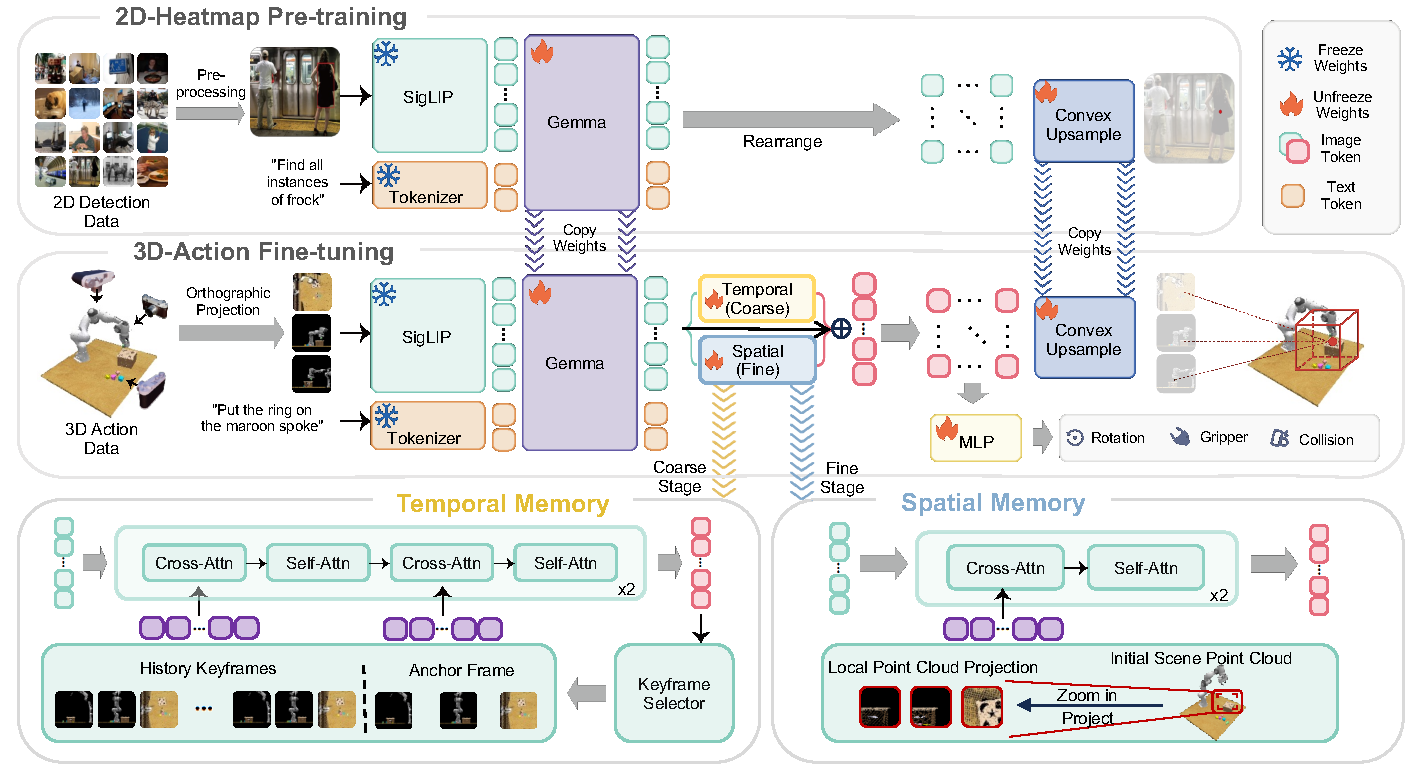
\includegraphics[width=\textwidth]{figures/architecture.pdf}
  \caption{\textbf{Model Architecture.}
  \textbf{Top:} \method first learns language-conditioned 2D heatmap prediction
  from detection data and transfers the resulting weights to 3D action
  fine-tuning. During a policy forward pass, the observed point cloud is
  rendered into orthographic views and processed with the language instruction
  by the VLM to produce multi-view visual tokens and heatmaps. The coarse
  heatmaps localize a 3D waypoint, around which the point cloud is cropped,
  magnified, and re-rendered for a shared-weight fine pass. The fine heatmaps
  determine the final translation, while global tokens and local tokens at the
  coarse waypoint are fed to an MLP to predict rotation, gripper state, and
  collision avoidance. \textbf{Bottom:} \memmethod augments this forward flow
  with temporal and spatial memories. At the coarse stage, the
  current tokens cross-attend to an anchor frame and selected historical
  keyframes to determine \emph{what to do next}. At the fine stage, they
  cross-attend to view-aligned spatial tokens obtained by re-rendering the
  initial point cloud under the current zoom, providing less-occluded geometry
  to determine \emph{where exactly to act}.}
  \label{fig:bridgevla_arch}
\end{figure*}

The key idea of \method is to align both the input and output of 3D
manipulation learning within a shared 2D space.
Specifically, \method formulates 3D manipulation as multi-view 2D heatmap
prediction.
A scalable pre-training stage first learns language-conditioned heatmap
grounding from large-scale 2D data
(Sec.~\ref{sec:bridgevla:pretrain}).
During downstream policy fine-tuning, the observed 3D scene is rendered into
multiple orthographic views, and the predicted heatmaps are back-projected
to recover the 3D end-effector translation of the next keyframe
(Sec.~\ref{sec:bridgevla:finetune}).
Fig.~\ref{fig:bridgevla_arch} provides an overview of the complete
framework, including the spatio-temporal memory extension introduced in
Sec.~\ref{sec:memmethod}.


\subsection{Problem Formulation}
\label{sec:bridgevla:problem}

We consider language-conditioned multi-task 3D manipulation learned from a
set of expert demonstrations
$\mathcal{D}=\{\tau^i\}_{i=1}^{N}$.
Each demonstration is represented as
\begin{equation}
    \tau^i =
    \left(
        l^i,
        \left\{
            \left(\mathbf{o}_t^i,\mathbf{a}_t^i\right)
        \right\}_{t=1}^{H_i}
    \right),
\end{equation}
where $l^i$ is a language instruction,
$\mathbf{o}_t^i$ is the observation at step $t$, and
$\mathbf{a}_t^i$ is the corresponding expert action.
The observation $\mathbf{o}_t$ consists of one or more RGB-D images captured
by calibrated cameras.

Following prior keyframe-based manipulation methods
\cite{johns2021coarse,shridhar2023perceiver,goyal2023rvt},
the policy is queried at a sparse set of decision points and predicts the
end-effector configuration of the next keyframe.
For single-arm manipulation, the action is represented as
\begin{equation}
    \mathbf{a}_t =
    \left(
        \mathbf{x}_t,
        \mathbf{R}_t,
        g_t,
        c_t
    \right),
    \label{eq:action}
\end{equation}
where $\mathbf{x}_t\in\mathbb{R}^{3}$ is the target end-effector
translation, $\mathbf{R}_t\in SO(3)$ is the target rotation,
$g_t\in\{0,1\}$ denotes the gripper state, and
$c_t\in\{0,1\}$ is a collision-avoidance flag used by the motion planner.
The collision flag is omitted for benchmarks that do not provide this
action component.

The original \method learns a language-conditioned policy that predicts the
next best pose from the current observation:
\begin{equation}
    \mathbf{a}_t =
    \pi_{\mathrm{B}}
    \left(
        \mathbf{o}_t,l
    \right).
    \label{eq:bridgevla_policy}
\end{equation}
After each prediction, a motion planner or benchmark-specific low-level
controller executes the target action.
The observation is then refreshed, and the policy predicts the next
keyframe.
This process continues until task completion or a predefined step limit is
reached.

Equation~\eqref{eq:bridgevla_policy} defines the memory-free formulation of
\method, in which each action is predicted from the current observation
alone.
Sec.~\ref{sec:memmethod} extends this formulation by conditioning the
policy on information retained from earlier interactions.


\subsection{2D-Heatmap Pre-Training}
\label{sec:bridgevla:pretrain}

The original VLM backbone is pre-trained to generate token sequences, whose
outputs do not directly preserve the spatial structure required for precise
robot action prediction.
To align VLM pre-training with downstream policy learning, we introduce an
additional pre-training stage that teaches the model to ground
language-specified objects through 2D heatmap prediction.

We use the 120K object-detection split of
RoboPoint~\cite{yuan2024robopoint} as the pre-training dataset.
Each training sample consists of an image, a text prompt describing one or
more objects of interest, and the bounding boxes of the corresponding
objects.
For each target object $i$, we construct a spatially truncated Gaussian
probability map:
\begin{equation}
H_i^{\mathrm{gt}}(\mathbf{x})
=
\begin{cases}
p_i(\mathbf{x}),
&
p_i(\mathbf{x}) \geq p_{\min},
\\
0,
&
\text{otherwise},
\end{cases}
\label{eq:single_object_probability_map}
\end{equation}
where $\mathbf{x}=(u,v)$ denotes a pixel location and
\begin{equation}
p_i(\mathbf{x})
=
\exp
\left(
-\frac{
\left\|
\mathbf{x}-\widehat{\mathbf{x}}_i
\right\|_2^2
}{
2\sigma^2
}
\right).
\end{equation}
Here, $\widehat{\mathbf{x}}_i$ is the center of the bounding box of object
$i$, $\sigma$ controls the spatial extent of the Gaussian, and $p_{\min}$
is the truncation threshold.

When multiple target objects are specified in the same prompt, their
probability maps are averaged and normalized to construct the final
ground-truth heatmap:
\begin{equation}
H_{\mathrm{avg}}(\mathbf{x})
=
\frac{1}{N_{\mathrm{obj}}}
\sum_{i=1}^{N_{\mathrm{obj}}}
H_i^{\mathrm{gt}}(\mathbf{x}),
\end{equation}
\begin{equation}
H^{\mathrm{gt}}(\mathbf{x})
=
\frac{
H_{\mathrm{avg}}(\mathbf{x})
}{
\sum_{\mathbf{x}'\in\Omega}
H_{\mathrm{avg}}(\mathbf{x}')
},
\label{eq:multi_object_probability_map}
\end{equation}
where $N_{\mathrm{obj}}$ is the number of target objects and $\Omega$
denotes the image domain.
Examples of the resulting heatmap annotations are shown in
Fig.~\ref{fig:pretrain_dataset}.

As illustrated in Fig.~\ref{fig:bridgevla_arch}, the input image and the
text prompt describing the objects of interest are jointly processed by the
VLM backbone.
We employ PaliGemma~\cite{beyer2024paligemma}, which consists of a SigLIP
vision encoder~\cite{zhai2023sigmoid} and a Gemma transformer
backbone~\cite{team2024gemma}.
PaliGemma is originally pre-trained to take one or more images together with
a prefix text and autoregressively generate a suffix text.
Although causal attention is used for suffix-token generation, image tokens
and prefix-text tokens interact through bidirectional attention.
Consequently, each output image token is conditioned on both the visual
observation and the language query.

To recover spatial structure from these output tokens, we rearrange the
image tokens according to their original patch positions, forming a
two-dimensional feature grid.
A convex-upsampling module~\cite{teed2020raft} then decodes this grid into a
heatmap with the same spatial resolution as the input image.
Unlike fixed interpolation operations such as bilinear or nearest-neighbor
upsampling, convex upsampling predicts spatially varying interpolation
weights, allowing the decoder to recover finer localization details.

The model is optimized using the cross-entropy loss
\begin{equation}
L_{\mathrm{pre}}
=
-\sum_{\mathbf{x}\in\Omega}
H^{\mathrm{gt}}(\mathbf{x})
\log
\widehat{H}(\mathbf{x}),
\label{eq:pretrain_heatmap_loss}
\end{equation}
where $\widehat{H}$ is the predicted heatmap after spatial softmax
normalization.

This pre-training stage changes the output interface of the VLM from
unstructured token generation to language-conditioned spatial localization.
Unlike 3D VLA methods that represent robot actions as token
sequences~\cite{zhen20243d,qu2025spatialvla}, our model produces a
spatially structured 2D heatmap.
The formulation is also scalable because any vision-language dataset whose
annotations can be converted into spatial targets, such as object centers,
keypoints, or segmentation regions, can in principle be used for
pre-training.
The resulting VLM backbone and heatmap decoder are subsequently transferred
to 3D action fine-tuning.


\subsection{3D Action Fine-Tuning}
\label{sec:bridgevla:finetune}

During downstream policy learning, \method preserves the 2D input and
heatmap-output interface established during pre-training while using
explicit 3D geometry for robot action prediction.

Given RGB-D images captured by one or more calibrated cameras, we first
reconstruct a colored point cloud of the observed scene.
Following RVT~\cite{goyal2023rvt} and
RVT-2~\cite{goyal2024rvt}, the point cloud is rendered into three
orthographic projection images corresponding to the top, front, and right
views.
The three rendered images and the language instruction are then processed
by the pre-trained VLM backbone to predict one translational heatmap for
each view.

Notably, the VLM operates purely on images and language: no proprioceptive
signals, such as robot joint states or end-effector poses, are fed into its
forward pass.
This design preserves the image--language input format used during
pre-training and reduces the distribution shift between 2D heatmap
pre-training and 3D policy fine-tuning.

\paragraph{Translation prediction}
To recover the translational action, we uniformly sample candidate 3D
locations within the robot workspace.
Each candidate location is projected onto the three orthographic views, and
its score is obtained by aggregating the corresponding heatmap values:
\begin{equation}
s_t(\mathbf{x})
=
\sum_{v=1}^{V}
\widehat{H}_{t,v}
\left(
\Pi_v(\mathbf{x})
\right),
\qquad V=3,
\label{eq:translation_score}
\end{equation}
where $\Pi_v$ denotes the projection onto view $v$, and
$\widehat{H}_{t,v}$ is the predicted heatmap for that view.
The candidate with the highest score is selected as the end-effector
translation of the next keyframe:
\begin{equation}
\widehat{\mathbf{x}}_t
=
\arg\max_{\mathbf{x}}
s_t(\mathbf{x}).
\label{eq:translation_prediction}
\end{equation}
This procedure preserves the geometric correspondence between the
multi-view observations, heatmap outputs, and 3D translational actions.

\paragraph{Rotation, gripper, and collision prediction}
The non-translational action components are predicted jointly from
multi-view features that combine global scene context with local evidence
around the predicted translation.
For each orthographic view, we obtain a global feature by max-pooling all
output image tokens.
We then project the predicted 3D translation onto the view and take the
output image token at this 2D location as the local feature.
The global and local features of the three views are concatenated and passed
to a single three-layer MLP, whose output vector is split into the rotation,
gripper, and collision-avoidance predictions.
We take these features only from the coarse stage, described next.

The end-effector rotation is represented in the continuous 6D form
of~\cite{zhou2019continuity}, from which the rotation matrix is recovered by
Gram--Schmidt orthonormalization.
The gripper state and collision-avoidance flag are each predicted by a
two-class softmax over a pair of logits.

\paragraph{Coarse-to-fine refinement}
A prediction over the complete workspace provides global localization but
may lack the precision required for fine-grained manipulation.
Following prior work~\cite{james2022coarse,goyal2024rvt}, \method adopts a
coarse-to-fine refinement strategy.

The first forward pass predicts a coarse translation from orthographic views
covering the complete workspace.
The point cloud is then cropped and magnified using a cuboid centered at the
predicted coarse translation.
A second set of orthographic images is rendered from this zoomed local point
cloud and processed by the same VLM backbone.
The translation predicted by the fine pass is used as the final
end-effector position for execution.
The coarse and fine passes share model parameters and differ only in the
spatial range represented by their input projections.

\paragraph{Fine-tuning objective}
The fine-tuning objective contains four components:
\begin{equation}
L_{\mathrm{base}}
=
L_{\mathrm{trans}}
+
L_{\mathrm{rot}}
+
L_{\mathrm{gripper}}
+
L_{\mathrm{collision}}.
\label{eq:base_loss}
\end{equation}

The translation loss $L_{\mathrm{trans}}$ supervises heatmap prediction
using cross-entropy.
For each orthographic view, the ground-truth translational heatmap is
constructed using the normalized single-target probability map defined in
Eq.~\eqref{eq:single_object_probability_map}, where
$\widehat{\mathbf{x}}_i$ becomes the projected pixel location of the
ground-truth end-effector translation at the next keyframe.
The loss is applied to heatmaps predicted at both coarse and fine
stages.

The rotation loss $L_{\mathrm{rot}}$ is the squared Frobenius norm of the
difference between the rotation matrix recovered from the predicted 6D
representation and the ground-truth rotation matrix.
The gripper and collision terms are two-class cross-entropy losses.
For benchmarks that do not provide a collision-avoidance label,
$L_{\mathrm{collision}}$ is omitted.

To improve geometric robustness, random rigid-body transformations are
applied jointly to the input point cloud and ground-truth action during
training.
Additional implementation and optimization details are provided in
Appendix~\ref{app:finetune_hparams}.

The coarse-to-fine design not only improves spatial precision, but also
exposes two complementary stages at which information from earlier
observations can be incorporated.
The coarse stage reasons over the complete workspace and determines the next
target region; it could therefore benefit from temporal context
about previous interactions and completed sub-goals.
The fine stage performs precise localization within a zoomed local crop,
where task-relevant geometry may be occluded by the robot or manipulated
objects; it could therefore benefit from a persistent spatial reference.

Motivated by this stage-specific decomposition, Sec.~\ref{sec:memmethod}
introduces \memmethod, which augments the coarse-stage representation with
temporal memory and the fine-stage representation with spatial memory.
The resulting framework extends \method from a policy conditioned only on
the current observation to a memory-conditioned policy, while preserving
its original heatmap-based action interface, action parameterization, and
input--output alignment.


\section{\memmethod}
\label{sec:memmethod}

\subsection{Overview}
\label{sec:memmethod:formulation}

The preceding section introduces \method as a memory-free policy that
predicts each action from the current observation and language instruction.
Although this formulation is effective for many manipulation tasks, the
current observation alone may be insufficient when the policy must track
previously completed sub-goals or utilize task-relevant geometry that becomes occluded during execution.

To address these limitations, we extend \method to a memory-conditioned
policy:
\begin{equation}
    \mathbf{a}_t
    =
    \pi_{\mathrm{M}}
    \left(
        \mathbf{o}_t,
        l,
        \mathcal{M}_t
    \right),
    \label{eq:mem_policy}
\end{equation}
where $\mathcal{M}_t$ denotes the episode memory available at decision step
$t$.
We decompose the memory into two complementary components:
\begin{equation}
    \mathcal{M}_t
    =
    \left(
        \mathcal{T}_t,
        \mathcal{S}_t
    \right),
    \label{eq:memory_decomposition}
\end{equation}
where $\mathcal{T}_t$ is a temporal memory that summarizes the interaction
history, and $\mathcal{S}_t$ is a spatial memory that preserves previously
observed scene geometry.

The two memories complement the coarse-to-fine action prediction of
\method.
Temporal memory is incorporated at the coarse stage to help the policy
determine \emph{what to do next} from the execution history.
Spatial memory is incorporated at the fine stage to help the policy
determine \emph{where exactly to act} when the target geometry is partially
occluded.
Both memories are represented and processed in the visual token space of the
VLM, allowing them to be integrated without modifying the original
heatmap-based action interface.


\subsection{Temporal Memory for Coarse-Stage Reasoning}
\label{sec:memmethod:temporal}

The coarse stage determines the approximate target region and provides the
features used to predict rotation, gripper state, and collision avoidance.
Because these decisions may depend on both recent interactions and overall
task progress, we augment the coarse-stage representation with temporal
memory.
We formulate the temporal memory as
\begin{equation}
    \mathcal{T}_t
    =
    \left(
        \mathbf{A}_0,
        \mathcal{H}^{\mathrm{nbr}}_t,
        \mathcal{H}^{\mathrm{sub}}_t
    \right),
    \label{eq:temporal_memory}
\end{equation}
where $\mathbf{A}_0$ denotes the initial anchor views,
$\mathcal{H}^{\mathrm{nbr}}_t$ contains recent neighboring keyframes, and
$\mathcal{H}^{\mathrm{sub}}_t$ contains adaptively selected sub-goal
keyframes.
All three components are stored as coarse-stage visual tokens.
Together, they provide a fixed reference to the initial scene, short-term
context about recent transitions, and longer-term evidence of completed
sub-goals.


\subsubsection{Initial Anchor Views}
\label{sec:memmethod:anchor}

At the beginning of each episode, the initial point cloud is rendered into
the same three orthographic views used by the coarse stage.
The resulting visual tokens are stored as $\mathbf{A}_0$.
Comparing the current representation with $\mathbf{A}_0$ helps the policy
identify scene changes that have occurred since the beginning of the
episode.
Because the coarse-stage virtual cameras remain fixed throughout execution,
the anchor views provide a consistent global reference for reasoning about
task progress.


\subsubsection{History Keyframes}
\label{sec:memmethod:bank}

The initial anchor captures changes relative to the beginning of the episode,
but does not describe the sequence of interactions that produced the current
state.
We therefore maintain a dynamic history buffer containing neighboring and
sub-goal keyframes.
The neighboring-keyframe memory
$\mathcal{H}^{\mathrm{nbr}}_t$ stores the most recent $n$ executed
keyframes, with $n=2$ in all our experiments.
It provides short-term context about recent state transitions.
The sub-goal-keyframe memory
$\mathcal{H}^{\mathrm{sub}}_t$ stores representative historical
observations selected by the adaptive module described in
Sec.~\ref{sec:memmethod:gate}.
These observations record informative milestones and provide longer-term
evidence of completed sub-goals.
Both types of keyframes are cached as coarse-stage visual tokens.
Together, they represent immediate interaction context and longer-term task
progress.
Memory capacity, frame ordering, and buffer-management details are provided
in Appendix~\ref{app:finetune_hparams}.


\subsubsection{Adaptive Sub-Goal Keyframe Selection}
\label{sec:memmethod:gate}

Storing every historical keyframe would introduce redundancy.
We therefore introduce a lightweight adaptive selection module
$D_{\phi}$ to determine whether the current keyframe contains
informative evidence of task progress to be retained in
$\mathcal{H}^{\mathrm{sub}}_t$.
A learnable query token attends to the image tokens after temporal-memory
integration and summarizes them into a single vector, from which a small MLP
predicts a retention probability.
A keyframe is retained when its predicted probability exceeds a predefined
threshold.
The selection module operates on the memory-conditioned tokens
rather than the tokens before memory integration.
This allows it to assess whether the current observation provides information
that is not already represented in $\mathcal{T}_t$, thereby preserving
informative milestones while avoiding redundant observations.

\subsection{Spatial Memory for Occlusion-Robust Fine Localization}
\label{sec:memmethod:spatial}

Temporal memory helps the coarse stage identify the next target region, but
does not directly help recover the fine-grained geometry required for precise
localization.
At the fine stage, the robot arm, gripper, or manipulated object may partially
occlude the target region in the current local crop.
For example, Fig.~\ref{fig:anchor_memory} shows a case in which the gripper
and grasped object obscure the target receptacle.

To provide a persistent geometric reference, we store the colored point cloud
of the initial observation as $\mathbf{P}_0$.
Because this observation is captured before substantial robot interaction,
it typically provides a less-occluded view of the workspace.
Unlike a fixed 2D image, the stored point cloud can be re-rendered using the
same viewpoint and zoom configuration as any subsequent fine-stage crop.
Once the coarse stage predicts a waypoint
$\widehat{\mathbf{x}}^{\mathrm{c}}_t$, we apply the same zoom operation to
the current point cloud and the stored reference $\mathbf{P}_0$.
The zoomed reference is then rendered through the fine-stage virtual cameras
and encoded into visual tokens:
\begin{equation}
    \mathcal{S}_t
    =
    \Phi
    \left(
        \mathrm{Render}
        \left(
            \mathrm{Zoom}
            \left(
                \mathbf{P}_0;
                \widehat{\mathbf{x}}^{\mathrm{c}}_t
            \right)
        \right)
    \right),
    \label{eq:spatial_memory}
\end{equation}
where $\Phi$ denotes the VLM backbone applied to the re-rendered views
together with the language instruction, and $\mathcal{S}_t$ is the spatial
memory associated with the current fine-stage crop.

\begin{figure}[t]
  \centering
  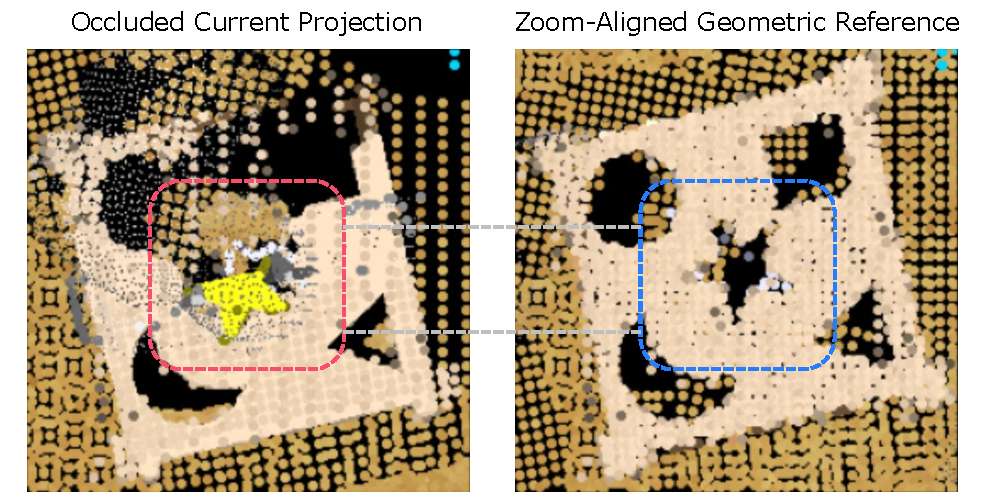
\includegraphics[width=\linewidth]{figures/anchor_memory.pdf}
  \caption{\textbf{Occlusion-robust fine localization using spatial
  memory.}
  \emph{Left:} the current zoomed observation, partially occluded by the
  gripper and manipulated object.
  \emph{Right:} the stored point cloud $\mathbf{P}_0$ re-rendered under
  the same predicted waypoint and zoom transformation, providing a
  spatially aligned, less-occluded reference of the same local region.}
  \label{fig:anchor_memory}
\end{figure}

Because the current local observation and the re-rendered spatial reference
share the same virtual camera configuration, they are geometrically aligned
at the view level.
Accordingly, we let tokens from each current view attend only to memory tokens from
the corresponding reference view.
The current observation represents the latest state of the scene, whereas
the spatial memory provides previously visible geometry that may now be
occluded.
Thus, the spatial memory complements rather than replaces the current
observation.
This adaptive zoom alignment enables a single canonical point cloud
$\mathbf{P}_0$ to provide spatial references for different local regions
throughout the episode.
Because the required crop depends on the current coarse waypoint,
$\mathcal{S}_t$ is rendered and encoded on demand at every decision step.


\subsection{Memory Integration}
\label{sec:memmethod:integration}

After constructing the temporal and spatial memories, we inject them into
the corresponding stages of \method using compact attention modules.
Temporal memory conditions the coarse-stage representation, whereas spatial
memory conditions the fine-stage representation.

To avoid repeatedly processing historical projection images, the temporal
buffer stores their encoded visual tokens rather than the raw images.
Each cached observation is represented by a token grid in
$\mathbb{R}^{V\times N\times d}$, where $V$ is the number of orthographic
views, $N$ is the number of visual tokens per view, and $d$ is the token
dimension.
These are the VLM backbone's language-conditioned output image tokens, 
and can be reused throughout the episode without re-encoding.

Let $\mathbf{Z}^{\mathrm{c}}_t$ and
$\mathbf{Z}^{\mathrm{f}}_t$ denote the current coarse- and fine-stage visual
tokens, respectively.
We obtain the memory-conditioned representations as
\begin{equation}
    \widetilde{\mathbf{Z}}^{\mathrm{c}}_t
    =
    F_{\mathrm{temp}}
    \left(
        \mathbf{Z}^{\mathrm{c}}_t,
        \mathcal{T}_t
    \right),
    \qquad
    \widetilde{\mathbf{Z}}^{\mathrm{f}}_t
    =
    F_{\mathrm{spa}}
    \left(
        \mathbf{Z}^{\mathrm{f}}_t,
        \mathcal{S}_t
    \right),
    \label{eq:memory_integration}
\end{equation}
where $F_{\mathrm{temp}}$ and $F_{\mathrm{spa}}$ denote the temporal and
spatial memory-injection modules.
Each block consists of two attention layers.
Within each layer, the current visual tokens serve as queries, while the
corresponding memory tokens serve as keys and values in cross-attention.
The retrieved information is subsequently fused with the current
representation through self-attention and feed-forward updates.
The output preserves the shape of the input token grid:
\begin{equation}
    \widetilde{\mathbf{Z}}^{s}_t
    \in
    \mathbb{R}^{V\times N\times d},
    \qquad
    s\in\{\mathrm{c},\mathrm{f}\}.
    \label{eq:memory_output_shape}
\end{equation}
Consequently, the convex-upsampling modules and action-prediction heads of
\method can be applied without modification.
The temporal and spatial memory-injection modules introduce approximately
168M and 84M parameters, respectively, while the adaptive sub-goal-selection
module introduces approximately 18M parameters.
Despite this modest architectural overhead, the memory modules substantially
improve performance on memory-dependent tasks, as evaluated in
Sec.~\ref{sec:experiments}.

\subsection{Bimanual Extension}
\label{sec:memmethod:bimanual}

The temporal and spatial memories encode the shared episode state and
workspace geometry rather than arm-specific information.
This scene-level formulation allows \memmethod to extend naturally to
bimanual manipulation with only lightweight modifications.
Specifically, we introduce arm-specific action heads by duplicating the
convex-upsampling module and the MLP-based action heads, while sharing the VLM backbone, temporal memory, spatial memory, and adaptive selection module between the two arms.
At the coarse stage, the arm-specific heads operate on the shared
memory-conditioned representation and predict a separate coarse waypoint
for each arm.
At the fine stage, each arm independently constructs a zoomed local crop
around its predicted coarse waypoint and refines its final translation.
The resulting bimanual action is represented as
\begin{equation}
    \mathbf{a}^{\mathrm{bi}}_t
    =
    \left(
        \mathbf{a}^{\mathrm{left}}_t,
        \mathbf{a}^{\mathrm{right}}_t
    \right),
    \label{eq:bimanual_action}
\end{equation}
where each arm-specific action follows the representation defined in
Eq.~\eqref{eq:action}.
This shared-trunk, arm-specific-head design successfully supports bimanual action prediction without duplicating the computationally expensive VLM backbone or the episodic memory modules.

\subsection{Training and Inference Details}
\label{sec:memmethod:training}

\subsubsection{Training}

During training, the temporal and spatial memories associated with each
sample are constructed from preceding observations in the corresponding
expert demonstration.
The initial observation provides the temporal anchor views and the spatial memory reference, while neighboring and annotated sub-goal keyframes are
selected from earlier execution steps.

To preserve geometric consistency, the random rigid-body augmentation
introduced in Sec.~\ref{sec:bridgevla:finetune} is applied consistently to
the current observation, the associated memory observations, and the
ground-truth actions.
The complete training objective is
\begin{equation}
    L
    =
    L_{\mathrm{base}}
    +
    \lambda_{\mathrm{check}}
    L_{\mathrm{check}},
    \label{eq:memory_training_loss}
\end{equation}
where $L_{\mathrm{base}}$ is the action-prediction loss defined in
Eq.~\eqref{eq:base_loss}, and $L_{\mathrm{check}}$ is a binary
cross-entropy loss that supervises whether the current keyframe should be retained as a sub-goal keyframe.
For bimanual tasks, $L_{\mathrm{base}}$ includes the action losses of both
arms, whereas the shared adaptive selection module is supervised once using
$L_{\mathrm{check}}$.


\subsubsection{Inference}

At the beginning of an episode, the initial observation is used to construct
the temporal anchor views and the spatial point-cloud reference
$\mathbf{P}_0$.
The remaining temporal-memory slots are initialized with zero padding.
After each executed action, the encoded image tokens of the current
observation are inserted into the temporal buffer as a neighboring
keyframe.
The adaptive selection module also determines whether the observation should
be retained as a sub-goal keyframe.
When the buffer exceeds its predefined capacity, the oldest entries are
removed according to the memory-management strategy described in
Appendix~\ref{app:finetune_hparams}.
Because temporal memory stores encoded image tokens rather than raw
projection images, historical observations do not require repeated visual encoding.
For spatial memory, we retain the colored point cloud of the initial observation and re-render and re-encode it at each decision step, since the required local crop depends on the dynamically predicted coarse waypoint. As only a single reference observation is processed, the resulting computational overhead remains low.
Overall, the memory extension introduces 269.77M additional parameters,
corresponding to a 9.2\% increase over the 2.92B-parameter backbone.
For the inference latency, \method\ takes 0.35 seconds per prediction step and \memmethod\ 0.57 seconds on a single NVIDIA RTX 4090 GPU, a gap that is minor compared with the observation transmission and motion execution that dominate each keyframe-based control step.